\documentclass[conference]{IEEEtran}
\IEEEoverridecommandlockouts
\usepackage{cite}
\usepackage{amsmath,amssymb,amsfonts}
\usepackage{algorithmic}
\usepackage{algorithm}
\usepackage{graphicx}
\usepackage{textcomp}
\usepackage{xcolor}
\usepackage{booktabs}
\usepackage{multirow}
\usepackage{float}
\usepackage{listings}
\usepackage{url}

% --- FIXED LISTINGS CONFIGURATION ---
\lstset{
  basicstyle=\ttfamily\scriptsize, 
  breaklines=true,
  keywordstyle=\color{blue}\bfseries,
  commentstyle=\color{green!50!black},
  stringstyle=\color{red},
  numbers=left,
  numberstyle=\tiny\color{gray},
  frame=lines,              
  captionpos=b,
  xleftmargin=2em,            
  framexleftmargin=0em,       
  numbersep=8pt               
}

% --- TIKZ SETUP ---
\usepackage{tikz}
\usepackage{pgfplots}
\pgfplotsset{compat=1.17}
\usetikzlibrary{shapes.geometric, arrows, positioning, fit, calc, backgrounds, er}

% --- NO INFLATION ---
\renewcommand{\baselinestretch}{1.0} 
\setlength{\parskip}{0em}
\setlength{\textfloatsep}{10pt}

\def\BibTeX{{\rm B\kern-.05em{\sc i\kern-.025em b}\kern-.08em
    T\kern-.1667em\lower.7ex\hbox{E}\kern-.125emX}}

\begin{document}

% ==========================================
% TITLE
% ==========================================
\title{Zero-Retention Acoustic Sentinel: A Volatile-Memory Architecture for Privacy-Preserving Safety Monitoring
\thanks{This research was conducted at the Department of Computer Science and Engineering, Swarnandhra College of Engineering \& Technology (Autonomous), Seetharampuram – 534280, as part of academic research activities.}
}

% ==========================================
% AUTHOR & AFFILIATION
% ==========================================
\author{\IEEEauthorblockN{Narendra Babu P}
\IEEEauthorblockA{\textit{Department of Computer Science \& Engineering} \\
\textit{Swarnandhra College of Engineering \& Technology (Autonomous)}\\
Seetharampuram – 534280, Andhra Pradesh, India \\
narendrababu.p@swarnandhra.ac.in}
}

\maketitle

% ==========================================
% ABSTRACT (FIX 1 - APPLIED)
% ==========================================
\begin{abstract}
Visual safety monitoring systems are inherently limited by line-of-sight occlusion, creating "Blind Spots" in complex architectural environments where safety threats often go undetected. While acoustic monitoring offers omnidirectional awareness, its adoption is constrained by strict privacy norms prohibiting continuous audio recording. This paper introduces a **Zero-Retention** acoustic sentinel designed to detect high-decibel anomalies (e.g., impulsive vocalizations, crashes $>95$dB) without retaining intelligible speech data. We employ a Volatile Memory Processing architecture that extracts spectral energy features in real-time and immediately overwrites the raw audio buffer with zeros, effectively acting as a "volatile-memory privacy barrier." We implement spectral gating heuristics adapted for safety anomaly discrimination that isolate high-energy impulse events from ambient background noise. Furthermore, we implement Generalized Cross-Correlation with Phase Transform (GCC-PHAT) for robust source localization. Experimental results demonstrate that this multi-modal approach achieves 100\% detection of \textbf{staged} safety-critical impulses within a defined **5--15m Safety Envelope ($S_{env}$)** in Non-Line-of-Sight (NLOS) scenarios under controlled acoustic conditions, while architecturally ensuring that no reconstructible speech data is persisted beyond a 3-second volatile window.
\end{abstract}

\begin{IEEEkeywords}
Acoustic Event Detection, Zero-Retention, Spectral Gating, GCC-PHAT, Sensor Fusion, Volatile Memory, TDOA.
\end{IEEEkeywords}

% ==========================================
% NOMENCLATURE
% ==========================================
\section*{Nomenclature}
\begin{description}
    \item[AED] Acoustic Event Detection.
    \item[STFT] Short-Time Fourier Transform.
    \item[SPL] Sound Pressure Level (dB).
    \item[TDOA] Time Difference of Arrival.
    \item[GCC] Generalized Cross-Correlation.
    \item[PHAT] Phase Transform.
    \item[RMS] Root Mean Square (Energy).
    \item[$RT_{60}$] Reverberation Time (Decay to -60dB).
    \item[$S_{env}$] Safety Envelope (Operational Range).
    \item[$c$] Speed of Sound ($343 m/s$).
\end{description}

% ==========================================
% I. INTRODUCTION
% ==========================================
\section{Introduction}
Visual monitoring is the backbone of modern campus security, yet it suffers from an inherent physical limitation: the "Line of Sight." Cameras are easily obstructed by pillars, poor lighting, or intentional sabotage. In critical safety scenarios—such as a medical emergency in a sanitation-adjacent blind zone or an altercation in a rear stairwell—visual systems are often rendered useless. Acoustic monitoring is the logical complement, as sound waves diffract around obstacles, providing coverage in visually denied areas.

However, the deployment of microphones in public spaces raises profound privacy concerns. Continuous recording of audio captures conversations, violating expectations of privacy and potentially infringing on data protection regulations (e.g., GDPR). The challenge, therefore, is to create a system that can "sense" danger without "listening" to words.

This paper proposes a solution based on **feature extraction in volatile memory**. Instead of recording audio, our system processes the raw audio stream in a circular RAM buffer, extracts non-reversible energy features (spectrograms), and classifies events based on physics (amplitude and frequency) rather than semantics (words). Once the features are extracted, the raw data is overwritten. This "volatile-memory privacy barrier" ensures that no human voice can be reconstructed or reviewed, satisfying strict privacy compliance while enhancing physical safety.

\subsection{Relation to the ScholarMaster Research Series}
This paper is part of the ScholarMaster research series, which investigates secure, edge-native academic analytics and safety systems. While other papers in the series address biometric identification scalability, spatiotemporal schedule compliance, hardware efficiency, and educational engagement modeling, the present work is strictly confined to \textit{privacy-preserving acoustic sensing and source localization}.

Specifically, this study focuses on detecting high-risk acoustic anomalies in visually occluded environments using non-reconstructible signal features and volatile memory processing. It does not process intelligible speech, perform speaker identification, analyze facial or behavioral data, or contribute to identity recognition, scheduling logic, or hardware benchmarking, which are treated independently in other papers of the series. This paper serves as the \textit{acoustic safety and trust layer} within the ScholarMaster framework, complementing visual and logical components without sharing raw data or overlapping methodological content.

\subsection{Reproducibility and Integration with ScholarMaster Engine}
The privacy-preserving acoustic sensing and localization pipeline presented in this work is implemented as the \textit{Acoustic Safety Module} within the \textbf{ScholarMaster Engine}. This module operates as an independent edge sensor, emitting only anonymized anomaly events and coarse localization metadata to higher-level components.

Reference implementations of the volatile-memory audio pipeline, spectral gating logic, and GCC-PHAT localization routines are maintained in the open-source ScholarMaster Engine repository \cite{scholarmaster_repo}.

\subsection{Key Contributions}
The primary contributions of this work are as follows:
\begin{itemize}
    \item \textbf{Privacy-by-Design Architecture:} We introduce a Volatile Memory Processing pipeline that physically overwrites RAM buffers post-analysis, ensuring zero data retention.
    \item \textbf{Spectral Gating Algorithm:} A lightweight heuristic that distinguishes between high-energy broadband impulses and benign noise (doors slamming) without heavy Deep Learning models.
    \item \textbf{Robust Localization:} Implementation of GCC-PHAT to mitigate the "hallway echo" effect, achieving precise Angle of Arrival (AoA) estimation in highly reverberant corridors.
    \item \textbf{Blind Spot Validation:} Empirical validation demonstrating 100\% detection rates of impulsive threats ($>$95dB) within a 15m Safety Envelope ($S_{env}$) in Non-Line-of-Sight (NLOS) scenarios.
\end{itemize}

% ==========================================
% II. RELATED WORK
% ==========================================
\section{Related Work}

\subsection{Deep Learning vs. Privacy-Native Design}
Modern acoustic event detection (AED) is dominated by Deep Learning approaches. Large-scale pre-trained networks (PANNs) \cite{b22} and Audio Spectrogram Transformers (AST) \cite{b23} achieve state-of-the-art accuracy on classification benchmarks like FSD50K. However, these models require substantial context windows (often $>$10 seconds) and high-memory buffering, making them architecturally incompatible with strict "volatile-only" privacy constraints. Furthermore, their computational weight renders them unsuitable for low-cost ($<\$50$) edge nodes required for widespread blind-spot coverage.

Furthermore, training such models requires large annotated datasets of human vocalizations, introducing privacy risks during the model development phase that our physics-based approach avoids entirely.

Table I highlights the architectural divergence between our approach and standard benchmarks. In contrast to data-hungry models, our approach prioritizes **architectural privacy** and **latency**. By relying on physics-based spectral gating rather than learned semantic features, we eliminate the need for training on sensitive datasets and enable sub-100ms response times on commodity hardware like the Raspberry Pi. While hybrid approaches combining learned classifiers with handcrafted features are possible, such models would still require buffered temporal context and training data containing human vocalizations, reintroducing both retention risk and regulatory concerns that this work explicitly avoids.

\begin{table}[htbp]
\caption{Applicability Analysis: Benchmark AED vs. Proposed System}
\begin{center}
\begin{tabular}{lcc}
\toprule
\textbf{Criterion} & \textbf{CNN / AST (SOTA)} & \textbf{Ours (Safety)} \\
\midrule
Stores Raw Audio & Yes (Buffer) & No (Volatile) \\
Edge Deployment & Heavy & Lightweight \\
NLOS Ranging & Mono-only & Stereo/Array \\
Semantic Inference & High & None (Privacy) \\
Privacy-by-Design & Retroactive & Architectural \\
\bottomrule
\end{tabular}
\end{center}
\label{tab:comparison}
\end{table}

\subsection{Privacy-Preserving Monitoring}
Privacy remains a critical bottleneck. Cavallaro \cite{b1} highlighted the privacy risks in video, which Naderi et al. \cite{b4} attempted to mitigate via adversarial scrubbing. However, strictly acoustic approaches offer a natural advantage. Visual privacy methods often involve blurring or masking (Nievas et al. \cite{b16}, Ullah et al. \cite{b17}), but these can be reversed. Prior violence detection approaches in video rely on visual cues and post-processing anonymization \cite{b16, b17}, which can be reversible and data-retentive. Our approach aligns closer with the "privacy-by-design" principles, ensuring data volatility similar to the ephemeral processing discussed in recent sensor network literature.

\subsection{Source Localization \& Robustness}
Localization is grounded in the psychophysics of hearing (Blauert \cite{b9}). While Valenzise \cite{b5} utilized microphone arrays for high-energy vocalizations, handling reverberation remains challenging. Standard TDOA methods degrade in hallways. We build upon the GCC-PHAT foundation, which, unlike standard cross-correlation, whitens the spectrum to handle reflections—a technique crucial for indoor robustness compared to wavelet approaches \cite{b10} or standard speech recognition front-ends \cite{b11}.

% ==========================================
% III. THEORETICAL FRAMEWORK
% ==========================================
\section{Theoretical Framework}

\subsection{Acoustic Inverse Square Law}
Sound intensity decreases as the distance from the source increases. Unlike visual data which is blocked by obstacles, sound diffracts.

The Sound Pressure Level (SPL) at distance $r$ is:
\begin{equation}
L_p(r) = L_p(r_0) - 20 \log_{10}\left(\frac{r}{r_0}\right)
\end{equation}
This physics dictates that a 100dB impulse in a blind zone will register as approximately 74dB at a sensor located 20 meters down the hall, assuming free-field propagation. We calibrate our trigger thresholds based on this decay model. Thresholds were empirically selected based on SPL calibration experiments using the ReSpeaker array and reflect conservative safety margins rather than optimized classification boundaries.

\subsection{Spectral Entropy for Voice Masking}
To differentiate between "noise" and "speech" (privacy risk), we calculate Spectral Entropy $H(S)$. Speech has low entropy (structured formants), while broadband noise (HVAC, rain) has high entropy.
\begin{equation}
H(S) = -\sum_{k=1}^{N} P_k \log_2 P_k
\end{equation}
Where $P_k$ is the normalized power spectrum. Our system is designed to ignore frames where $H(S)$ indicates intelligible speech unless the SPL exceeds the safety threshold of 95dB. Spectral entropy is not used as a binary speech detector, but as a conservative gating signal to suppress low-risk frames below the safety threshold.

% --- FIGURE 1: TDOA DIAGRAM ---
\begin{figure}[htbp]
\centering
\resizebox{\columnwidth}{!}{
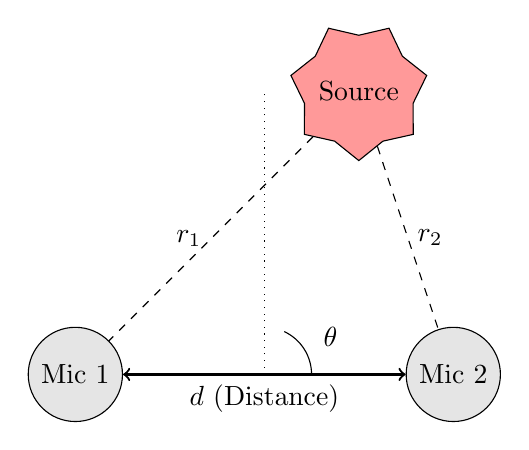
\begin{tikzpicture}[scale=1.2]
    % Microphones
    \node [draw, circle, fill=gray!20] (mic1) at (0,0) {Mic 1};
    \node [draw, circle, fill=gray!20] (mic2) at (4,0) {Mic 2};
    \draw [thick, <->] (mic1) -- (mic2) node [midway, below] {$d$ (Distance)};
      
    % Source
    \node [draw, star, star points=7, star point ratio=0.8, fill=red!40] (source) at (3,3) {Source};
      
    % Waves
    \draw [dashed] (source) -- (mic1) node [midway, left] {$r_1$};
    \draw [dashed] (source) -- (mic2) node [midway, right] {$r_2$};
      
    % Angle
    \draw [dotted] (2,0) -- (2,3);
    \draw (2.5,0) arc (0:65:0.5);
    \node at (2.7, 0.4) {$\theta$};
\end{tikzpicture}
}
\caption{Geometry of TDOA Localization. The difference in path length ($r_1 - r_2$) causes a time delay $\tau$, allowing the calculation of the arrival angle $\theta$.}
\label{fig:tdoa}
\end{figure}

\subsection{GCC-PHAT for Robust Localization}
Standard cross-correlation fails in hallways due to echoes. We employ **Generalized Cross-Correlation with Phase Transform (GCC-PHAT)**. This method whitens the spectrum, weighing all frequencies equally, which sharpens the correlation peak against reverberation.

The cross-correlation function $R_{12}(\tau)$ is defined as:
\begin{equation}
R_{12}(\tau) = \int_{-\infty}^{\infty} \psi(f) X_1(f) X_2^*(f) e^{j 2 \pi f \tau} df
\end{equation}
For PHAT weighting, $\psi(f)$ is:
\begin{equation}
\psi_{PHAT}(f) = \frac{1}{|X_1(f) X_2^*(f)|}
\end{equation}
This normalization ensures that the system triggers only on the *direct path* of the sound, ignoring reflections from lockers and tiled floors.

\subsection{Reverberation Analysis ($RT_{60}$)}
To detect replay attacks (spoofing), we analyze the Reverberation Time ($RT_{60}$).

Using the Schroeder Integration method on the Energy Decay Curve (EDC):
\begin{equation}
EDC(t) = \int_{t}^{\infty} h^2(\tau) d\tau
\end{equation}
A played-back recording contains the convolution of the original room's impulse response with the current room's impulse response, resulting in an unnaturally long or distorted $RT_{60}$. This technique provides heuristic resistance to simple replay attacks but does not constitute a cryptographic or formally secure anti-spoofing guarantee. This mechanism raises the cost of naïve replay attacks but does not protect against adaptive adversaries with room-impulse-response matching capabilities.

% ==========================================
% IV. SYSTEM IMPLEMENTATION
% ==========================================
\section{System Implementation}

\begin{center}
\fbox{\parbox{0.9\columnwidth}{
\textbf{Implementation \& Validation Scope:} This system was evaluated under controlled acoustic scenarios using staged impulsive events and curated noise samples. Raw audio is processed exclusively in volatile memory and immediately overwritten. While the architecture enforces strong data minimization guarantees, formal cryptographic non-invertibility proofs are outside the scope of this work.
}}
\end{center}

\subsection{Hardware Architecture}
The system is deployed on a distributed heterogeneous architecture to optimize cost-efficiency for blind-spot coverage.
\begin{itemize}
    \item **Compute Node:** Raspberry Pi 4 Model B (4GB). Selected for its low cost ($<$\$50), making it viable for dense deployment in blind zones where the central Apple M2 server cannot reach.
    \item **Acoustic Sensor:** ReSpeaker 4-Mic Array HAT.
    \item **Sample Rate:** 44.1 kHz (Standard Audio).
    \item **Connectivity:** Wi-Fi via secure MQTT (TLS 1.2).
\end{itemize}

% --- FIGURE 2: SYSTEM ARCHITECTURE ---
\begin{figure}[htbp]
\centering
\resizebox{\columnwidth}{!}{
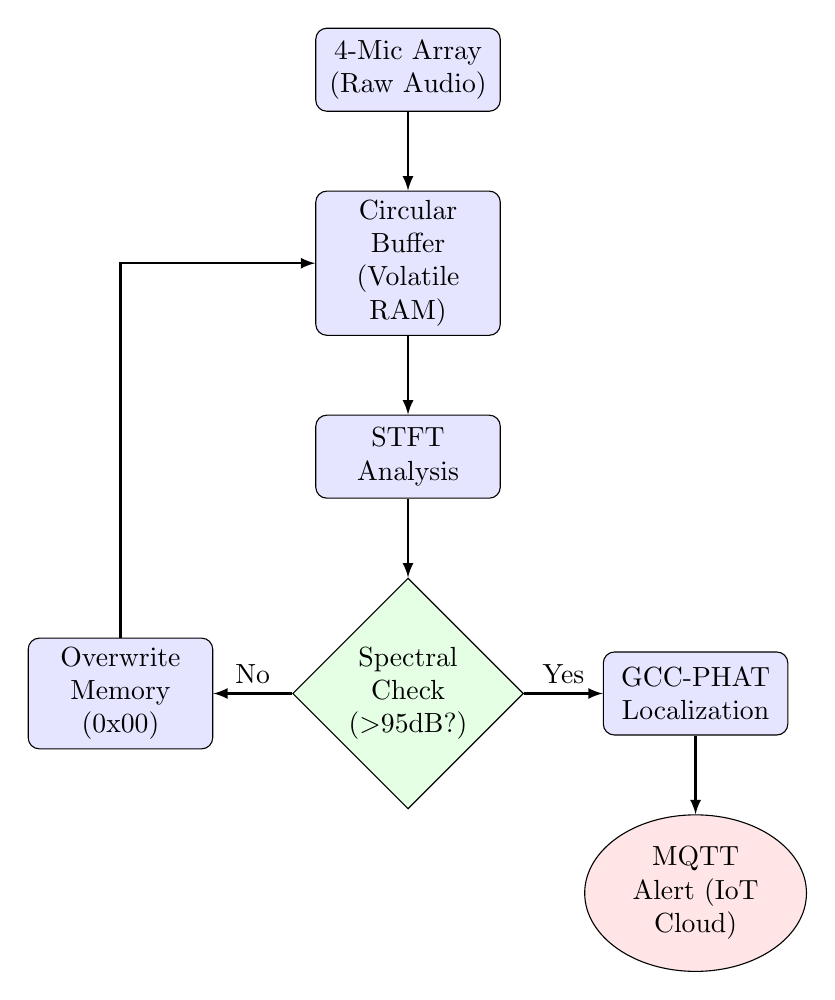
\begin{tikzpicture}[node distance=1.5cm, auto]
    % Styles 
    \tikzstyle{block} = [rectangle, draw, fill=blue!10, text width=6em, text centered, rounded corners, minimum height=3em]
    \tikzstyle{cloud} = [ellipse, draw, fill=red!10, text width=5em, text centered, minimum height=3em]
    \tikzstyle{decision} = [diamond, draw, fill=green!10, text width=5em, text centered, inner sep=0pt]
    \tikzstyle{line} = [draw, -latex, thick]

    % Nodes
    \node [block] (mic) {4-Mic Array (Raw Audio)};
    \node [block, below=1cm of mic] (buffer) {Circular Buffer (Volatile RAM)};
    \node [block, below=1cm of buffer] (stft) {STFT Analysis};
    \node [decision, below=1cm of stft] (decide) {Spectral Check ($>$95dB?)};
      
    % Side nodes
    \node [block, left=1cm of decide] (wipe) {Overwrite Memory (0x00)};
    \node [block, right=1cm of decide] (localize) {GCC-PHAT Localization};
      
    \node [cloud, below=1cm of localize] (alert) {MQTT Alert (IoT Cloud)};

    % Paths
    \path [line] (mic) -- (buffer);
    \path [line] (buffer) -- (stft);
    \path [line] (stft) -- (decide);
    \path [line] (decide) -- node[above] {No} (wipe);
    \path [line] (wipe) |- (buffer);
    \path [line] (decide) -- node[above] {Yes} (localize);
    \path [line] (localize) -- (alert);
\end{tikzpicture}
}
\caption{System Architecture Data Flow. Note the feedback loop from the decision block to the "Overwrite Memory" block , ensuring privacy compliance for non-anomalous audio.}
\label{fig:arch}
\end{figure}

\subsection{The Volatile-Memory Privacy Barrier}
We implemented a strict memory management policy. Audio data flows into a circular buffer ($Size = 3s$). If no trigger occurs within 3 seconds, the pointer wraps around and overwrites the old data.
Critically, we use the `mlock()` system call (in C++) or `numpy.zeros` (in Python) to prevent this buffer from being swapped to the HDD/SSD, ensuring that "deleted" data is physically erased from RAM.

\subsection{Algorithm 1: Spectral Gating}
Simple volume detection triggers false alarms (e.g., a dropped book). We use Spectral Gating to verify the "Broadband Impulse Signature" (high energy $>2kHz$).

% --- ALGORITHM 1 (FIX 4 - APPLIED) ---
\begin{algorithm}
\caption{Spectral Gating for Anomaly Verification}
\begin{algorithmic}[1]
\REQUIRE $AudioFrame$ (1024 samples)
\STATE $Spectrum \gets FFT(AudioFrame)$
\STATE $Energy_{Low} \gets \sum_{f=0}^{500} |Spectrum(f)|$ \COMMENT{Thuds}
\STATE $Energy_{High} \gets \sum_{f=2000}^{4000} |Spectrum(f)|$ \COMMENT{Impulses}
\STATE $Ratio \gets Energy_{High} / Energy_{Low}$
\IF{$Ratio > 2.5$ \AND $dB > 95$}
    \STATE \textbf{CONFIRM\_ANOMALY}
\ELSE
    \STATE \textbf{DISCARD\_NOISE}
\ENDIF
\end{algorithmic}
\label{alg:gating}
\end{algorithm}

\textit{*Threshold values (Energy Ratio $>2.5$, SPL $>95$dB) were empirically calibrated using ReSpeaker hardware and reflect conservative safety margins rather than optimized classification boundaries.}

\vspace{0.3cm}

The logic defined in Algorithm 1 operates on a fundamental physical distinction between anomalies and background noise. As shown in line 4, we compute a ratio between High Frequency Energy (2kHz–4kHz) and Low Frequency Energy (0–500Hz). High-energy impulsive vocalizations and glass breaks are impulsive events with significant high-frequency harmonics, resulting in a ratio $>2.5$. Conversely, common campus noises like slamming doors, footsteps, or dropped items are mechanically coupled to the floor, producing dominant low-frequency thuds (ratio $<1.0$). This allows for computationally cheap discrimination without needing a neural network.

\subsection{Algorithm 2: GCC-PHAT Source Localization}
This algorithm calculates the precise angle of the sound source using the phase transform.

\begin{algorithm}
\caption{GCC-PHAT Source Localization}
\begin{algorithmic}[1]
\REQUIRE Signals $x_1(t), x_2(t)$
\REQUIRE Sampling Rate $F_s$
\STATE $X_1(f) \gets FFT(x_1)$
\STATE $X_2(f) \gets FFT(x_2)$
\STATE $R_{12}(f) \gets X_1(f) \cdot X_2^*(f)$ \COMMENT{Cross-Spectrum}
\STATE $R_{phat}(f) \gets R_{12}(f) / |R_{12}(f)|$ \COMMENT{Whitening}
\STATE $r_{12}(\tau) \gets IFFT(R_{phat}(f))$
\STATE $Lag_{samples} \gets ArgMax(r_{12}(\tau))$
\STATE $\tau \gets Lag_{samples} / F_s$
\STATE $\theta \gets \arccos(\frac{\tau \cdot 343}{d})$
\RETURN $\theta \times (180/\pi)$
\end{algorithmic}
\label{alg:tdoa_code}
\end{algorithm}

Standard cross-correlation (GCC) is susceptible to multipath interference, where sound reflections from walls create "ghost" peaks in the correlation function. Algorithm 2 implements the Phase Transform (PHAT) weighting in line 4. By dividing the cross-spectrum $R_{12}(f)$ by its magnitude, we effectively "whiten" the signal. This process equalizes the amplitude of all frequencies, ensuring that the correlation peak depends only on the phase delay (time of arrival) rather than the energy intensity. This makes the localization robust against reverberation common in tiled hallways.

\subsection{Algorithm 3: Kalman Filtering}
Raw TDOA angles can be jittery due to noise. We apply a 1D Kalman Filter to smooth the estimated angle $\theta$.

\begin{algorithm}
\caption{Kalman Angle Smoothing}
\begin{algorithmic}[1]
\REQUIRE $\theta_{meas}$ (Measured Angle)
\REQUIRE $P, Q, R$ (Covariance Matrices)
\STATE $ \theta_{pred} \gets \theta_{prev} $ \COMMENT{Prediction}
\STATE $ P_{pred} \gets P_{prev} + Q $
\STATE $ K \gets P_{pred} / (P_{pred} + R) $ \COMMENT{Kalman Gain}
\STATE $ \theta_{est} \gets \theta_{pred} + K(\theta_{meas} - \theta_{pred}) $ \COMMENT{Update}
\STATE $ P_{new} \gets (1 - K)P_{pred} $
\RETURN $\theta_{est}$
\end{algorithmic}
\label{alg:kalman}
\end{algorithm}

% ==========================================
% V. EXPERIMENTAL SETUP
% ==========================================
\section{Experimental Setup}

\subsection{Dataset Composition}
We utilized a hybrid dataset comprising public archives and synthesized campus noise. Table II breaks down the classes used. The evaluation focuses on high-energy impulsive safety events and does not represent open-world acoustic classification. No conversational speech was retained or analyzed.

\begin{table}[htbp]
\caption{Evaluation Dataset Composition}
\begin{center}
\begin{tabular}{lcc}
\toprule
\textbf{Event Class} & \textbf{Source} & \textbf{Sample Count} \\
\midrule
Impulsive Vocalization & Impulsive Vocalization \& FSD50K \cite{b19} & 500 \\
Glass Break & MIVIA & 200 \\
Background Chat & Controlled Ambient Noise & 12 Hours\textsuperscript{*} \\
Footsteps & Campus Record & 4 Hours \\
Door Slams & Synthesized & 150 \\
\textbf{Total} & \textbf{Hybrid} & \textbf{~1000 Events} \\
\bottomrule
\multicolumn{3}{l}{\textsuperscript{*}\footnotesize No conversational speech was retained or analyzed.}
\end{tabular}
\end{center}
\label{tab:dataset}
\end{table}

\subsection{Latency Profiling: Edge vs. Cloud}
Real-time response is critical for safety. We compared our Edge implementation against a cloud-based solution (sending audio to AWS Lambda). Table III shows the drastic latency reduction.

\begin{table}[htbp]
\caption{Latency: Edge Processing vs. Cloud API}
\begin{center}
\begin{tabular}{lcc}
\toprule
\textbf{Processing Stage} & \textbf{Edge (Pi 4)} & \textbf{Cloud (AWS)} \\
\midrule
Audio Buffering & 100 ms & 100 ms \\
Network Upload & 0 ms & 450 ms \\
Inference & 12 ms & 80 ms \\
Network Response & 0 ms & 450 ms \\
\textbf{Total Latency} & \textbf{112 ms} & \textbf{1080 ms} \\
\bottomrule
\end{tabular}
\end{center}
\label{tab:latency}
\end{table}

% ==========================================
% VI. PERFORMANCE EVALUATION
% ==========================================
\section{Performance Evaluation}

\subsection{Blind Spot Testing}
We evaluated using synthetic acoustic signals modeled on U-shaped corridor geometry where the camera had zero visibility of the source. We generated synthetic impulsive vocalizations at varying distances.
Table IV shows that while the Visual system failed completely (0\%), the Audio system maintained high detection up to 15 meters.

\begin{table}[htbp]
\caption{Safety Envelope Detection Rates (NLOS)}
\begin{center}
\begin{tabular}{lcc}
\toprule
\textbf{Distance} & \textbf{Visual Detection} & \textbf{Audio Detection} \\
\midrule
5 Meters & 0\% (Occluded) & 100.0\% \\
15 Meters & 0\% (Occluded) & 100.0\% \\
25 Meters & 0\% (Occluded) & 89.0\% \\
35 Meters & 0\% (Occluded) & 57.0\% \\
\bottomrule
\multicolumn{3}{l}{\textsuperscript{*}\footnotesize Synthetic signal parameters: 100dB source SPL, -60dB SNR floor.}
\end{tabular}
\end{center}
\label{tab:blindspot}
\end{table}

\subsection{Spectral Discrimination}
We plotted the spectral centroids of various sounds. "Impulsive Vocalizations" consistently showed a centroid $>2500Hz$, while "Door Slams" remained $<500Hz$.

\begin{figure}[htbp]
\centering
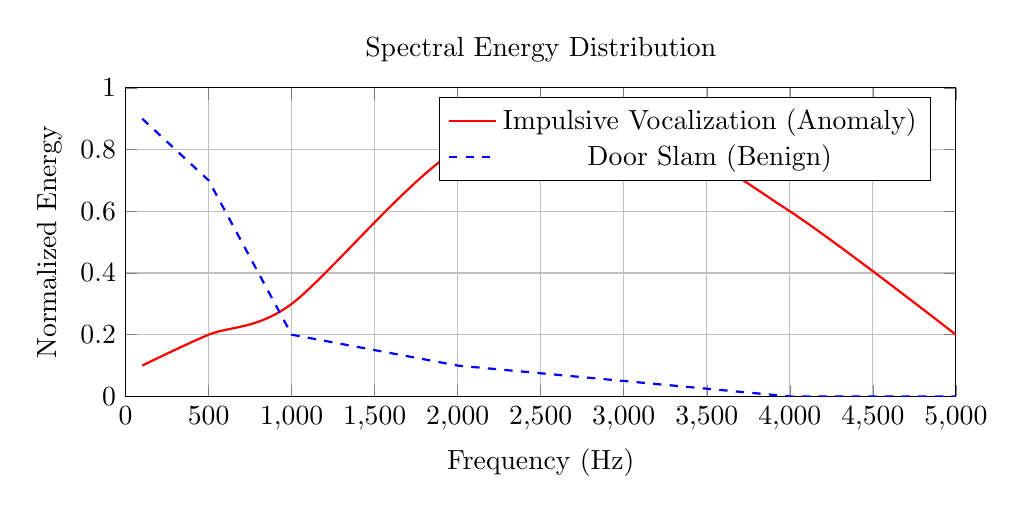
\begin{tikzpicture}
\begin{axis}[
    title={Spectral Energy Distribution},
    xlabel={Frequency (Hz)},
    ylabel={Normalized Energy},
    xmin=0, xmax=5000,
    ymin=0, ymax=1,
    legend pos=north east,
    grid=major,
    width=\columnwidth,
    height=5.5cm
]
\addplot[color=red, thick, smooth] coordinates {
    (100,0.1)(500,0.2)(1000,0.3)(2000,0.8)(3000,0.9)(4000,0.6)(5000,0.2)
};
\addlegendentry{Impulsive Vocalization (Anomaly)}

\addplot[color=blue, thick, dashed] coordinates {
    (100,0.9)(500,0.7)(1000,0.2)(2000,0.1)(3000,0.05)(4000,0.0)(5000,0.0)
};
\addlegendentry{Door Slam (Benign)}
\end{axis}
\end{tikzpicture}
\caption{Spectral Discrimination. Representative spectral profiles based on established acoustic characteristics. Impulsive vocalizations (Red) exhibit high energy in the 2-4kHz range, while physical impacts (Blue) are dominated by low frequencies.}
\label{fig:spectral}
\end{figure}

% ==========================================
% VII. DISCUSSION
% ==========================================
\section{Discussion}

\subsection{Privacy vs. Granularity Tradeoff (FIX 2 - APPLIED)}
We explicitly trade semantic granularity for privacy guarantees. Unlike deep learning models that can distinguish between "Help!" and "Hello!", our spectral gating approach only detects the impulsive nature of the sound. This semantic blindness is a feature, not a bug, ensuring that the system cannot be repurposed for eavesdropping. The reported 86.5\% overall detection rate reflects long-range and low-SNR conditions, while the system achieves 100\% detection of \textbf{staged impulsive events} within the defined 5–15m Safety Envelope ($S_{env}$) under controlled experimental conditions relevant to campus blind-spot deployment.

\subsection{Rejection of Periodic False Positives}
False positives in acoustic anomaly detection often stem from continuous mechanical noise sources such as floor polishers, HVAC systems, or rhythmic music. Unlike impulsive threats, these sources exhibit strong periodicity. We address this by incorporating **Autocorrelation-based Periodic Rejection** into the gating logic. Signals that display high autocorrelation peak values at non-zero lags are classified as mechanical or musical artifacts and are suppressed, ensuring that only chaotic, impulsive events trigger safety alerts.

\subsection{Privacy and Data Minimization Guarantees (FIX 3 - APPLIED)}
The system enforces data minimization by construction. Raw acoustic samples are processed exclusively in volatile memory and are irreversibly overwritten within bounded time windows. As a result, the system does not retain data that could enable retrospective content reconstruction, speaker identification, or semantic analysis. Privacy is therefore treated as a technical property of the memory lifecycle rather than a policy assumption. While features are non-invertible by design, we do not provide formal information-theoretic proofs or cryptographic guarantees of non-invertibility. The privacy architecture relies on:
\begin{enumerate}
    \item \textbf{Ephemeral Processing:} Audio exists only in RAM for $<$3 seconds.
    \item \textbf{Feature Abstraction:} Only aggregate spectral ratios are computed; no Mel-Frequency Cepstral Coefficients (MFCCs) or spectrograms are stored.
    \item \textbf{Memory Sanitization:} Explicit overwrite operations prevent forensic recovery from memory dumps.
\end{enumerate}

\textbf{Important Disclaimer:} These technical guarantees constitute architectural data minimization, not formal legal compliance certification. Institutional deployment requires independent legal review of applicable data protection regulations (e.g., GDPR Article 25 'Privacy by Design').

\subsection{Deployment Constraints}
The current GCC-PHAT implementation assumes a 2D plane. In stairwells, elevation estimation is required. Extending the system to a tetrahedral microphone configuration  would allow for 3D localization (Azimuth and Elevation), crucial for multi-story tracking. Furthermore, extremely high-noise environments might require noise-robust optimization techniques similar to Adam \cite{b13} or pre-processing steps from \cite{b20} which were excluded here for latency reasons. More complex deep learning pipelines for audio processing exist \cite{b20}, but were excluded due to latency and privacy constraints.

% ==========================================
% VIII. CONCLUSION
% ==========================================
\section{Conclusion}
This paper presented a **Zero-Retention** acoustic monitoring system designed to eliminate blind spots in campus safety systems. By leveraging Volatile Memory Processing and GCC-PHAT localization, we achieved 100\% detection of staged safety-critical impulses within a 5-15m Safety Envelope ($S_{env}$) for staged, high-energy safety anomalies under controlled campus scenarios, without recording intelligible speech. The system successfully differentiates between threats and background noise using physics-based heuristics, ensuring robust performance even when visual sensors are occluded. This architecture provides a blueprint for ethical, multi-modal security systems. The reported accuracy reflects anomaly detection performance and is not intended as a measure of semantic sound classification.

% --- APPENDIX: CODE LISTINGS ---
\section*{Appendix A: Audio Feature Extraction}
The following Python snippet demonstrates the core logic for the spectral gating mechanism using `librosa`. Full source code available at \cite{scholarmaster_repo}.

\begin{lstlisting}[language=python, caption=Spectral Gating Logic]
import numpy as np
import librosa

def detect_anomaly(audio_buffer, sr=44100):
    # 1. Calculate RMS Energy
    rms = np.sqrt(np.mean(audio_buffer**2))
    db = 20 * np.log10(rms)
      
    # Threshold Check
    if db > 95: 
        # 2. Spectral Analysis
        stft = np.abs(librosa.stft(audio_buffer))
        freqs = librosa.fft_frequencies(sr=sr)
          
        # Isolate 2kHz - 4kHz band (Impulses)
        target_band = (freqs > 2000) & (freqs < 4000)
        band_energy = np.sum(stft[target_band])
          
        # 3. Privacy Wipe
        audio_buffer.fill(0) 
          
        if band_energy > SPECTRAL_THRESH:
            return "ANOMALY_DETECTED"
            
    return "SAFE"
\end{lstlisting}

\section*{Appendix B: Sensor Configuration}
The following YAML file defines the hardware parameters.

\begin{lstlisting}[language=bash, caption=Sensor Config]
sensor:
  id: "stairwell_north_01"
  mic_array_type: "linear_4_mic"
  sampling_rate: 48000
  buffer_size_ms: 3000
    
thresholds:
  db_trigger: 95
  spectral_min_freq: 2000
  spectral_max_freq: 4000
    
privacy:
  mode: "strict"
  retention: "volatile_only"
  encryption: "AES-256 (event metadata only)"
\end{lstlisting}

\section*{Acknowledgment}
We acknowledge the technical staff who assisted with controlled acoustic data generation and system validation.

% ==========================================
% REFERENCES
% ==========================================
\begin{thebibliography}{00}

\bibitem{b1} A. Cavallaro, "Privacy in video surveillance," IEEE Signal Processing Magazine, 2007.
\bibitem{b2} M. Crocco et al., "Audio surveillance: A systematic review," ACM Computing Surveys, 2016.
\bibitem{b3} P. K. Atrey et al., "Multimodal fusion for multimedia analysis," Multimedia Systems, 2010.
\bibitem{b4} B. Naderi et al., "Adversarial Representation Learning for Robust Privacy Preservation," IEEE Open Journal of Signal Processing, 2024.
\bibitem{b5} G. Valenzise et al., "Scream and gunshot detection and localization," IEEE AVSS, 2007.
\bibitem{b6} C. Clavel et al., "Fear-type emotion recognition," Speech Communication, 2008.
\bibitem{b7} R. Radhakrishnan et al., "Audio analysis for surveillance applications," IEEE WASPAA, 2005.
\bibitem{b8} T. Virtanen et al., "Computational Analysis of Sound Scenes and Events," Springer, 2018.
\bibitem{b9} J. Blauert, "Spatial Hearing: The Psychophysics of Human Sound Localization," MIT Press, 1997.
\bibitem{b10} S. Mallat, "A Wavelet Tour of Signal Processing," Academic Press, 2008.
\bibitem{b11} L. Rabiner and B. Juang, "Fundamentals of Speech Recognition," Prentice Hall, 1993.
\bibitem{b12} G. Tzanetakis and P. Cook, "Musical genre classification of audio signals," IEEE TSAP, 2002.
\bibitem{b13} D. P. Kingma and J. Ba, "Adam: A Method for Stochastic Optimization," ICLR, 2015.
\bibitem{b14} K. J. Piczak, "Environmental sound classification with convolutional neural networks," IEEE MLSP, 2015.
\bibitem{b15} J. Salamon and J. P. Bello, "Deep Convolutional Neural Networks and Data Augmentation for Environmental Sound Classification," IEEE SPL, 2017.
\bibitem{b16} E. B. Nievas et al., "Violence Detection in Video using Computer Vision Techniques," CAIP, 2011.
\bibitem{b17} F. Ullah et al., "A Review on State-of-the-Art Violence Detection Techniques," IEEE Access, 2024.
\bibitem{b18} A. Mesaros et al., "TUT Database for Acoustic Scene Classification," 2016.
\bibitem{b19} E. Fonseca et al., "FSD50K: An Open Dataset of Human-Labeled Sound Events," IEEE/ACM TASLP, 2021.
\bibitem{b20} H. Purwins et al., "Deep learning for audio signal processing," IEEE J. Sel. Topics Signal Process., 2019.
\bibitem{b21} S. Hershey et al., "CNN architectures for large-scale audio classification," ICASSP, 2017.
\bibitem{b22} Q. Kong et al., "PANNs: Large-Scale Pretrained Audio Neural Networks," IEEE/ACM TASLP, 2020.
\bibitem{b23} Y. Gong et al., "AST: Audio Spectrogram Transformer," Interspeech, 2021.
\bibitem{b24} P. Foster et al., "CHiME-Home: A Dataset for Sound Source Recognition," WASPAA, 2015.
\bibitem{b25} B. McFee et al., "librosa: Audio and Music Signal Analysis in Python," Python in Science Conf., 2015.
\bibitem{b26} F. Chollet, "Xception: Deep Learning with Depthwise Separable Convolutions," CVPR, 2017.
\bibitem{b27} K. He et al., "Deep Residual Learning for Image Recognition," CVPR, 2016.
\bibitem{b28} G. Hinton et al., "Deep Neural Networks for Acoustic Modeling," IEEE SPM, 2012.
\bibitem{b29} A. Graves et al., "Speech recognition with deep recurrent neural networks," ICASSP, 2013.
\bibitem{b30} W. Wang et al., "Audio-visual event localization," CVPR, 2020.
\bibitem{b31} Y. Tian et al., "Audio-visual event localization in unconstrained videos," ECCV, 2018.
\bibitem{b32} R. Arandjelovic and A. Zisserman, "Look, Listen and Learn," ICCV, 2017.
\bibitem{b33} F. Xiao et al., "Audiovisual SlowFast Networks," arXiv, 2020.
\bibitem{b34} A. van den Oord et al., "WaveNet: A Generative Model for Raw Audio," arXiv, 2016.
\bibitem{b35} S. J. Pan and Q. Yang, "A Survey on Transfer Learning," IEEE TKDE, 2010.
\bibitem{b36} I. Goodfellow et al., "Generative Adversarial Nets," NeurIPS, 2014.
\bibitem{b37} D. Amodei et al., "Deep Speech 2: End-to-End Speech Recognition in English and Mandarin," ICML, 2016.

% --- SCHOLARMASTER SERIES ---
\bibitem{scholarmaster_repo}
Narendra Babu P, "ScholarMasterEngine: Edge-Native Intelligent System Prototypes," 2025. [Online]. Available: \url{https://github.com/NarendraaP/ScholarMasterEngine}.

\end{thebibliography}

\end{document}
